\chapter{Experimento}
\label{experimento}

Nesta seção será apresentada como foi realizado o experimento de implementação de uma RSSF em um ambiente de Smart Building, utilizando o padrão IEEE 802.15.4g SUN. A finalidade deste experimento é avaliar as performance da rede analisando valores de RSSI e PDR obtidos.

O experimento foi realizado em um dos prédios do campus Campina Grande do IFPB, Instituto Federal de Educação, Ciência e Tecnologia da Paraíba. Sendo este constituído principalmente de salas de escritório e de alguns laboratórios, possuindo 4 andares separados por grossos pisos de concreto. Este cenário é particularmente desafiador para um enlace sem fio pois não é possível ter uma linha de visada entre o transmissor e o receptor além de apresentar muito ocorrência de propagação por múltiplos caminhos e pode apresentar fácilmente áreas de sombreamentos de sinais.

\section{Visão Geral}
\label{subsec:visaogeral}
Como demonstrado na figura \ref{fig:rede_visão_geral}, a rede foi composta por 11 dispositivos transmissores, denominado pelo restante do texto como Tx, que enviavam três replicas de mensagens, uma replica para cada modulação do padrão IEEE 802.15.4g SUN. Três receptores, denominado pelo restante do texto como Rx, foram configurados para receber mensagens em apenas uma das modulações do padrão. Os dispositivos Rx, conectados a um computador, enviavam as mensagens recebidas pelo rádio para a porta serial. O computador utiliza um sistema operacional baseado em GNU/Linux e executa um script Python que lê as mensagens seriais enviadas pelos dispositivos Rx, estruturava os dados no formato JSON e os persistia no banco de dados InfluxDB.

\begin{figure}[h]
    \begin{center}
        \caption{Visão Geral da Rede}
        \includegraphics[width=0.8\textwidth]{./sections/textual/chapters/images/rede_visão_geral.png}\\
        Fonte autoral
        \label{fig:rede_visão_geral}
    \end{center}
\end{figure}

Os dispositivos Tx foram espalhados pelos quatro andares do prédio, posicionados em canaletas, como demonstrado na figura \ref{fig:tx_canaleta}, e no interior de uma sala. Enquanto que os dispositivos Rx foram colocados no interior do laboratório GComPI, presente no primeiro piso do prédio.

\begin{figure}[h]
    \begin{center}
        \caption{Exemplo de Local dos Dispositivos Tx}
        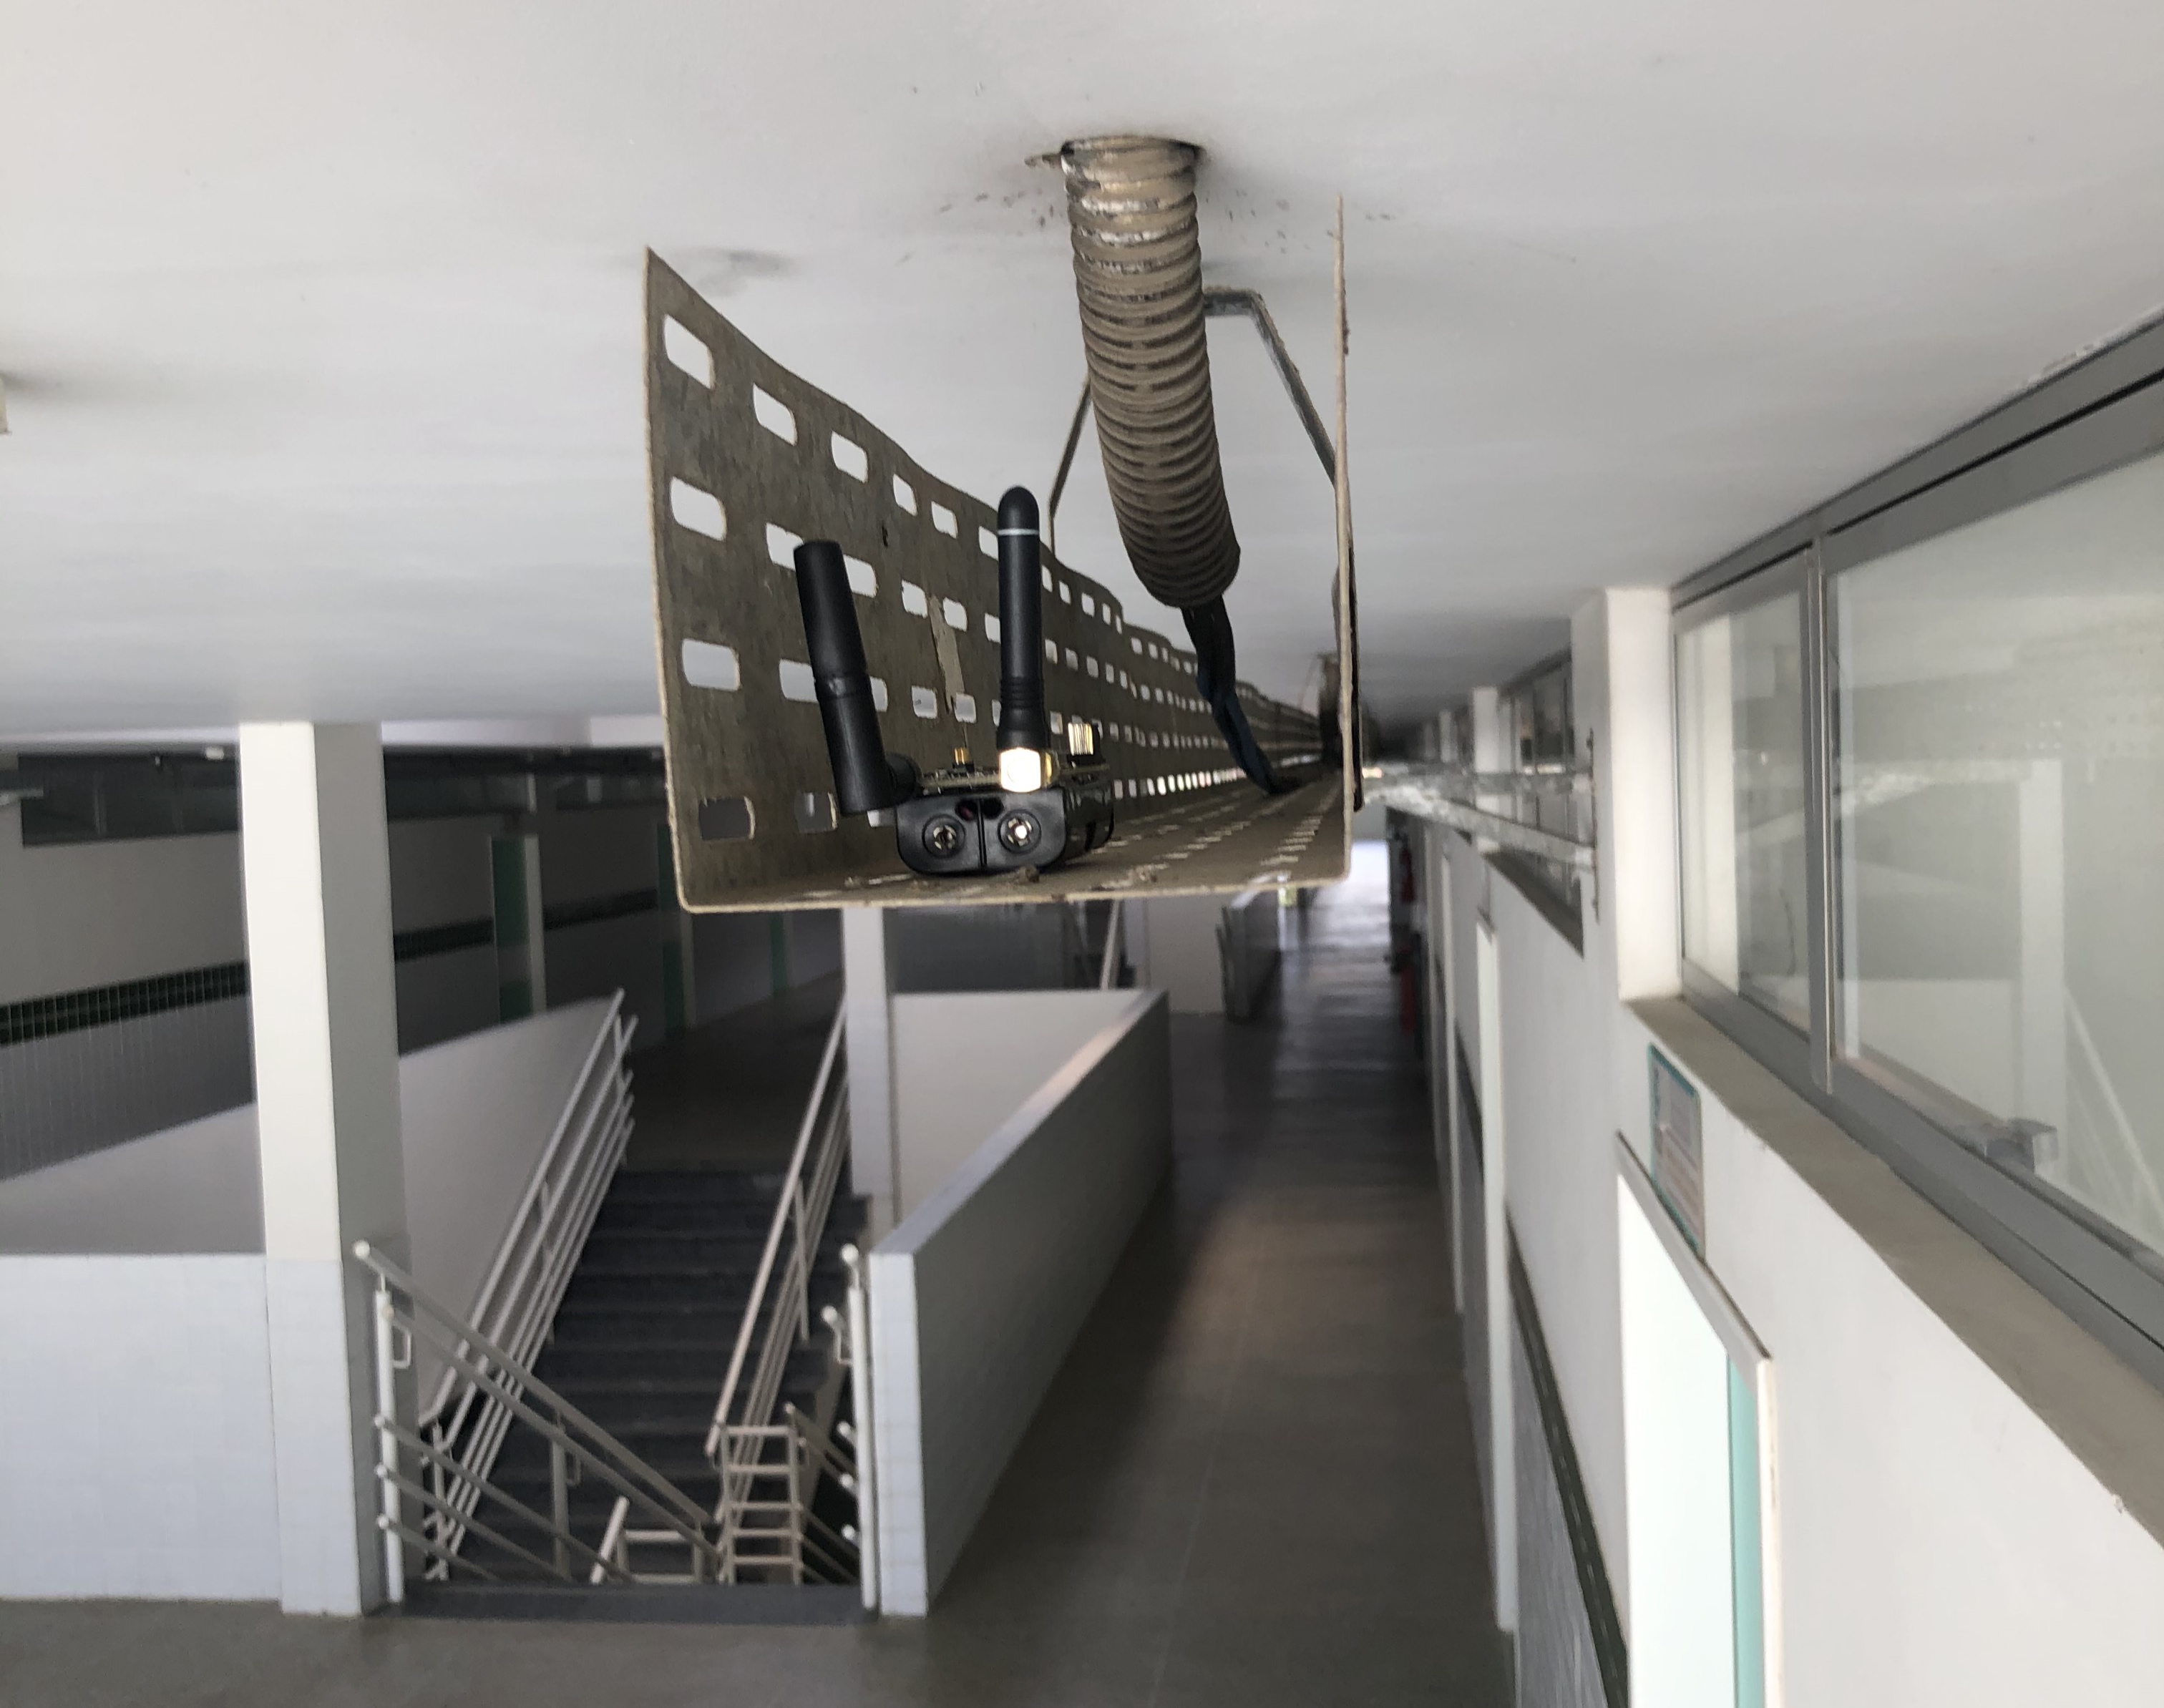
\includegraphics[width=10cm]{./sections/textual/chapters/images/tx_canaleta.jpg}\\
        Fonte autoral
        \label{fig:tx_canaleta}
    \end{center}
\end{figure}

\section{Openmote B}
O OpenMote B é um hardware de desenvolvimento e prototipação de plataformas IoT. Contém o processador SoC, \emph{System-on-Chip}(Sistema em um \emph{Chip}), CC2535 da Texas Instruments, constituído de um ARM Cortex-M3, com 32 K\emph{bytes} de memoria RAM e 512 K\emph{bytes} de memoria Flash. Neste processador também vem embarcado um transceptor com suporte ao padrão IEEE 802.15.4 que utiliza a modulação DSSS-OQPSK na faixa ISM de 2,4GHz. Possui também o transceptor AT86RF215 da ATMEL que implementa as três configurações do padrão IEEE 802.15.4g nas faixas ISM abaixo das faixas 1GHz e na faixa ISM 2,4GHz \cite{openmoteb-userguide}.

Para a realização do experimento, o código base do firmware dos dispositivos está presente no repositório \cite{openmoteb-firmware}. Foram realizadas alterações ao código base e estão disponíveis no repositório \cite{openmoteb-gcompi}.

\section{Transmissão dos dados}
Na tabela \ref{table:config} estão descritos as configurações de operação de cada modulação.
\begin{table}[h!]
    \centering
    \begin{tabular}{|c c c c|}
        \hline
        Modulação & SUN-FSK & SUN-OQPSK & SUN-OFDM \\ [0.5ex]
        \hline\hline
        \makecell{Taxa de                          \\transmissão(K\emph{bit}/s)    } & 50      & 50                       & 50       \\\hline
        \makecell{Tipo de                          \\Modulação                     } & BFSK    & OQPSK                    & BPSK     \\\hline
        \makecell{Índice de                        \\Modulação                   } & 1.0     & N/A                      & N/A      \\\hline
        \makecell{Taxa de \emph{Chips}             \\(k\emph{chips}/s) } &         & 100                      & N/A      \\\hline
        \makecell{Modo de                          \\Espalhamento                  } & N/A     & \makecell{SHR:(32,1)-DSS            \\ PHR:(8,1)-DSS\\ PSDU:none} & N/A      \\\hline
        \makecell{Frequência                       \\Central (MHz)              } & 902,2   & 904                      & 902,8    \\\hline
        \makecell{Largura de                       \\banda do canal                                                               \\(MHz)        } & 0,2     & 2000                     & 0,8      \\\hline
        \makecell{Canais                           \\disponíveis                    } & 129     & 12                       & 31       \\\hline
        \makecell{Potência de                      \\Transmissão (dBm)         } & 15      & 15                       & 9        \\\hline
        \makecell{Sensibilidade de                 \\Recepção (dBm)       } & -114    & -116                     & -111     \\\hline
        \makecell{Limiar do CCA                    \\(dBm)                   } & -94     & -93                      & -91      \\ \hline
        \hline
    \end{tabular}
    \caption{Configurações utilizadas de cada modulação.}
    \label{table:config}
\end{table}

Os dispositivos foram configurados para realizar, a cada minuto, três ciclos de envio de mensagens, como representado na figura \ref{fig:ciclo_envio}, em cada ciclo é transmitido três mensagens, uma para cada modulação do padrão. A cada envio de mensagem o dispositivo espera 50 ms e a cada ciclo de envio o dispositivo espera 100 ms, do primeiro para o segundo ciclo, ou 200 ms, do segundo para o terceiro ciclo. Ao realizar os três ciclos de transmissão, o dispositivo entra em modo \emph{sleep} por 58250 ms totalizando assim 60 segundos para o envio de nove mensagens, foi calculado que cada transmissão (com uma carga útil de 32 \emph{bytes}) leva 100 ms para ser totalmente transmitido.

\begin{figure}[h]
    \centering
    \caption{Ciclo de Envio de Mensagens.}
    
\includegraphics[width=\textwidth]{./sections/textual/chapters/images/metodo_ciclo_envio.png}\\
    Fonte autoral
    \label{fig:ciclo_envio}
\end{figure}

Cada mensagem transmitida é constituída dos seguintes campos:
\begin{itemize}
    \item Identificador do dispositivo: um campo de 6 \emph{bytes} que registra uma letra entre ``a'' e ``k'' que identifica cada um dos onze dispositivos Tx;
    \item Identificador de pacote: um campo de 8 \emph{bytes} que registra um contador que é também a identificação do pacote;
    \item Identificador da modulação: um campo de 1 \emph{byte} que registra em qual modulação o pacote foi enviado;
    \item Identificador de Pacote do Transmissor: um campo de 1 \emph{byte} que registra em qual dos ciclos de transmissão, ciclo um, dois ou três, o pacote foi enviado;
    \item Quantidade de Tentativas do CSMA: um campo de 1 \emph{byte} que registra quantas vezes o transmissor sensoreou o canal de radiofrequência antes de realizar a transmissão, o valor pode ir de 1 até 3, caso chegue na terceira tentativa o dispositivo não realiza a transmissão;
    \item Valor de RSSI do transmissor: um campo de 1 \emph{byte} que registra o valor de energia do canal. Se o valor estiver acima do valor apresentado no campo ``Limiar do CCA'' na tabela \ref{table:config} o dispositivo espera um tempo aleatório, em ms, e realiza outra tentativa de transmissão.
\end{itemize}

Para completar os 32 \emph{bytes} de carga útil cada mensagem foi preenchida com 14 \emph{bytes}.

\section{Recepção e Persistência dos dados}
Os dispositivos Rx, recebiam um total de 99 mensagens por minuto, 9 para cada dispositivo Tx. A cada recepção de mensagem, é verificada o valor de RSSI da transmissão e adicionada ao final da sequências de \emph{bytes} recebida. A sequência é então encaminhada para a saída sérial do dispositivo Rx.

No \emph{gateway} foi implementado um \emph{script Python}, disponível no repositório \cite{openmoteb-serialReader}, responsável por verificar continuamente as portas seriais do computador, para receber as mensagens dos dispositivos Rx. Uma vez recebida, a mensagem é estruturada em um dicionario \emph{python}, uma estrutura de dados de chave valor. A mensagem estruturada era então gravada em um banco de dados chamado InfluxDB que utiliza series temporais como índice de dados, ou seja, cada mensagem é salva de acordo com horário da transmissão.